% catalogue: title = Background layer via main/background names
% catalogue: min-coverage = 0.40
\documentclass[border=10pt]{standalone}
\PassOptionsToPackage{dvipsnames,svgnames,x11names}{xcolor}
\usepackage{tikz}
\usepackage{pgfplots}
\pgfplotsset{compat=newest}
\usepgfplotslibrary{groupplots}
\usetikzlibrary{arrows.meta}
\begin{document}
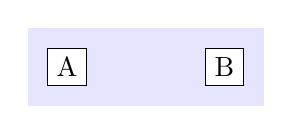
\begin{tikzpicture}
    \pgfdeclarelayer{background}
    \pgfsetlayers{background,main}
    \node[draw, fill=white] (a) at (0, 0) {A};
    \node[draw, fill=white] (b) at (2, 0) {B};
    \begin{pgfonlayer}{background}
        \fill[blue!10] (-0.5, -0.5) rectangle (2.5, 0.5);
    \end{pgfonlayer}
\end{tikzpicture}
\end{document}
